% \documentclass{report}

% \usepackage{subcaption} % package for subfigures
% \usepackage{hyperref}  % package for linking figures etc
% \usepackage{enumitem}  % package for description with bullets
% \usepackage{graphicx}  % package for importing images
% \usepackage{mathtools} % package for math equation
% \usepackage{mathrsfs}  % package for math font
% \usepackage{indentfirst} % package for getting ident after section or paragraph
% \usepackage[export]{adjustbox}
% % \usepackage{amsmath}

% \setlength{\parindent}{2em} % how much indent to use when we start a paragraph

% \graphicspath{ {./theory/figures/} }       % path for images

% \begin{document}

\chapter{Introduction}
Nowadays, the enormous increase of computing power help us deal with a lot of difficult situations appeared in our daily life.
A lot of areas of science have managed to tackle with problems, which were consided non trivial 20 years ago. One of
these area is Computer Vision and an important problem is human action recognition and localization.
\section{Problem statement}
The area of human action recognition and locatization has 2 main goals:
\begin{enumerate}
\item Automatically detect and classify any human activity, which appears in a video.
\item Automatically locate in the video, where the previous action is performed.
\end{enumerate}

\subsection{Human Action Recognition}
Considering human action recognition, a video may be consisted of only by 1 person doing something. However, this is a ideal
situation. In most cases, videos contain multiple people, who perform multiple actions or may not act at all in some segments.
So, our goal is not only to classify an action, but to dertemine the temporal boundaries of each action.
\subsection{Human Action Localization}
Alongside with Human Action Recognition, another problem is to present spatial boundaries of each action. Usually, this means
presenting a 2D bounding box for each video frame, which contains the actor. Of course, this bounding box moves alongside with
the actor.

\section{Applications}
The field of Human Action Recognition and Localization has a lot of applications which include 
 content based video analysis,automated video segmentation, security and surveillance systems,
human-computer interaction.

The huge availability of data (especially of videos) create the  necessity to find ways to take advantage of them.
About 2.5 billion images are uploaded at Facebook database every month, more than 34K hours of video in YouTube and
about 5K images every minute. On top of that, there are about 30 million surveillance cameras in US, which means
about 700K video hours per day. All those data need to be seperated in categories according to their content in
order to search them more easily. This process takes place by hand, by a user who attaches
keywords or tags to each video. However, most users avoid doing that, so many videos end up without any tagging information.
This situation creates the need to create algorithms for automated indexing based on the content of the video.

Another application is video summury. This area take place usually in movies or sports events. In movies,
video analysis algorithms can create a small video containing all the important moments of the movie. This
can be achieved by choosing video segments which an important action takes place such as killing the villain
of the movie. In sports events, video summury applications include creating highlight videos automatically, like
a video containing all achieved goals in football match.

On top of that, human action recognition can replace human operators in surveillance systems. Until now,
security systems include a system of multiple cameras handled by a human operator, who judges if a person
is acting normally or not. Automatic action classification systems can act like human, and immediately
judge if there is any human behavioral anomaly.

Last but not least, another field of application is related with human-computer interaction. Robotic applications
help elderly people deal with their daily needs. Also, gaming applications using Kinect create new kinds of
gaming experience without the need of a physical game controller.

\section{Challenges and Datasets}
There are various types of human activities. Depending on their complexity, weconceptually categorize human activities into four different
levels: gestures, actions, interactions, and group activities. Gestures are elementary movements of a person’s body part, and are the atomic
components describing the meaningful motion of a person. ``Stretching an arm'' and ``raising a leg'' are good examples of gestures.
Actions are single person activities that may be composed of multiple gestures organized temporally, such as ``walking'', ``waving'', and
``punching''. Interactions are human activities that involve two or more persons and/or objects. For example, ``two persons fighting'' is
an interaction between two humans and ``a person stealing a suitcase from another'' is a human-object interaction involving two humans and one
object. Finally, group activities are the activities performed by conceptual groups composed of multiple persons and/or objects. ``A group of persons marching'', ``a group having a meeting'', and ``two groups fighting'' are typical examples of them.
The wide variety of human activities and applications creates a lot of challenges which involve action recognition systems.
The most important challenges include large variations in appearence of the actors, camera view-point changes, occlusions,
non-rigid camera motions etc. On top of that, a big problem is that there are too many action classes which means
that manual collection of training sample is prohibitive. Also, some times, action vocabulary is not well defined.
As figure \ref{fig:open_example} shows, ``Open'' action can include a lot of kinds of actions, so we must carefully
choose which granularity of the action we will consider.

\begin{figure}[h]
  \centering
  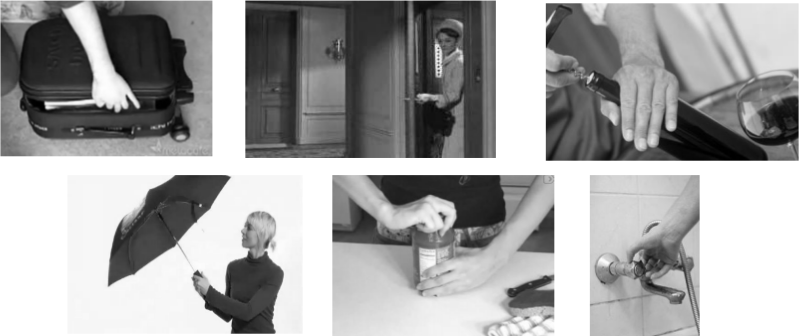
\includegraphics[scale=0.3]{open_example}
  \caption{Examples of ``Open'' action}
  \label{fig:open_example}

\end{figure}

In order to deal with those challenges, several standard action datasets have been created in order to delevop
robust human action recognition systems and detection algorithms.
The first datasets included 1 actor performing using a static camera over homogeneous backgrounds.
Even though, those datasets helped us design the first action recognition algorithms, they were not able to deal with the above
challenges.
This lead us to design datasets containing more ambigious videos, such as Joint-annotated Human Motion Database(JHMDB) (\cite{Kuehne11})
and UCF-101 (\cite{soomro2012ucf101}). These datasets contain only human actions, the second category presented above.

\subsection{JHMDB Dataset}
The JHMDB dataset (\cite{Jhuang:ICCV:2013}) is a fully annotated dataset for human actions and human poses. It is consisted of 21 action categories and 928
clips extracted from Human Motion Database (HMDB51) \cite{Kuehne11}. This dataset contains trimmed videos with duration between
15 to 40 frames. Each clip is annotated for each frame using a 2D pose and contains only 1 action.
In order to train our model for action localization, we modify 2D poses into 2D boxes containing the whole pose in each frame.
There are available 3 different splits for training data, proposed by the authors. We chose the first split which contains 660
videos for training set and 268 for validation . 

\subsection{UCF-101 Dataset}
The UCF-101 dataset (\cite{soomro2012ucf101}) contains 13320 videos from 101 action categories.
From those, for 24 classes and 3194 video spatio-temporal annotations are included. This means that there is a 2D bounding box surrounding the actor for each frame in which an action is taking place.
We seperate them in 2284 videos for training set and 910 for validation test according to the
first proposed training split. For training data, there are videos up to 641 frames, while in validation data max number of frames is 900.
Each video, both training and validation, is untrimmed, including sometimes more than 1 actions taking place simultaneously.
We took annotations from
\cite{singh2016online} because the by the authors proposed annotations contain some mistakes.

\section{Motivation ans Contibutions}
The current achievements in Object Recognition Networks and in 3D Convolution Networks for Action Recognition have triggered us to try
to combine them in order to achieve state-of-the-art results for action localization. We introduce a new network structure inspired by
\cite{DBLP:journals/corr/HouCS17}, \cite{DBLP:journals/corr/abs-1712-09184},\cite{Ren:2015:FRT:2969239.2969250} and for implementation
by \cite{jjfaster2rcnn}.

Our contributions are the following:
\begin{enumerate}
\item We create a new framework for action localization extending the code taken from faster RCNN implementation. Based on the structure
  proposed by \cite{DBLP:journals/corr/HouCS17}, we modified it, using a 3D Resnet34 instead of C3D, which previous approach used.

\item Furthermore, we proposed our own TPN Network, a Network for proposing candidate action tubes give a small video segment.
  Following the approach \cite{DBLP:journals/corr/HouCS17} proposed, we firstly implement an architecture which uses
  cubboids as anchors, which then using a regressor it becomes a sequence of bounding boxes, likely to contain an action.
  We experiment with two candidate regressor's architecture and proposed and implement a 3D RoiAlign which uses trilinear
  interpolation for extracting each proposed action tube's activation maps. 
  Inspired by \cite{DBLP:journals/corr/abs-1712-09184}, we proposed and implement a TPN which uses predefined sequences of bounding
  boxes as 3D anchors. We proposed anchors that last equal with and less than video segment's duration in order our architecture to be able to
  perform temporal localization.  we explore two different regressors' architectures for better spatial precision using activation
  maps extracted from 2D RoiAlign, treating each frame seperatly.
\item Inspired by liniking algorithm proposed by \cite{DBLP:journals/corr/HouCS17}, we introduce our own linking algorithm, which
  uses a combination of actioness and overlap scores in order to decide if 2 proposed action tubes would connect or not and some updatable lists.
  Our approach includes gathering all candidate action tubes whose score is bigger than a threshold, and use them as active action tubes for
  new possible connections. When the number of gathered active action tube is bigger than a threshold, we keep the k-best scoring action tubes
  and remove the rest.  We implement this algorithm using, also, CUDA code in order to calculate connection score faster. We proposed 3 versions of this algorith:
  \begin{enumerate}
  \item An approach which uses an updatable scoring threshold, in order not to calculate unnecessary connection scores
  \item An approach which doesn't use an updatable scoring threshold, but it just updateds ``active'' action tube more frequently.
  \item An approach which, also, uses NMS or softmax-NMS algorithms for getting wider action tube proposals.
  \end{enumerate}
  Also, we implement, from scratch, another connection algorithm proposed by \cite{DBLP:journals/corr/abs-1903-00304} and extending it in order to work for ToIs instead of frames, which they proposed.
  We modified our TPN structure in order to calculate progression and progress rate scores in order to calculate connection scores and generate candidate action tubes.
\item We experiment using several classifier in order to find the most suitable. We considered 2 feature maps extracted using 3D RoiAlign and proposed action tubes, without any other
  modification. Also, we explore the different ratios and number of groundtruth foreground tubes that should be used during training
  stage. Finally, we tried to perform only temporal localization using temporal information generated from proposed action tubes.
\end{enumerate}

\section{Thesis structure}
The rest of Thesis is organized as follows. Chapter 2 provides an general introduction to Machine Learning techniques currently used.
After that, we present the basic elements of object recognition systems and alongside with loss functions and evaluation metrics that
we used. Also, Chapter 2 presents an brief overview of literature on human action recognition and localization. Chapter 3 introduces the first basic element of our network, Tube Proposal Network (TPN), a network which proposes Tubes of Interest (ToIs), which are sequences of bounding boxes, with are likely to contain a performed action. Furthermore, it contains all the proposed architectures for achieving this.
Chapter 4 proposes algorithms for linking the proposed TOIs from every video segment and proposal performance is presented.
In Chapter 5, we present all the classification approaches we used for designing our architecture and some classification results.
Chapter 6 is used for conclusions, summary of our contribution alongside with possible future work.

% \end{document}
